
%% Circular Motion Questions used on the
%% NYSED Physics Regents Examination
%%--------------------------------------------------

%% this section contains 45 problems


%% Section June2014
%%--------------------
\element{nysed}{
\begin{question}{June2014-Q38}
    A \SI{1.0e3}{\kilo\gram} car travels at a constant speed of \SI{20}{\meter\per\second}.
    The diameter of the track is \SI{1.0e2}{\meter}.
    The magnitude of the car's centripetal acceleration is:
    \begin{multicols}{2}
    \begin{choices}
      \correctchoice{\SI{4.0}{\meter\per\second\squared}}
        \wrongchoice{\SI{0.20}{\meter\per\second\squared}}
        \wrongchoice{\SI{8.0}{\meter\per\second\squared}}
        \wrongchoice{\SI{2.0}{\meter\per\second\squared}}
    \end{choices}
    \end{multicols}
\end{question}
}

\element{nysed}{
\begin{question}{June2014-Q45}
    A body, $B$, is moving at constant speed in a horizontal circular path around point $P$.
    Which diagram shows the direction of the velocity ($v$) and the direction of the centripetal force ($F_c$) acting on the body?
    \begin{multicols}{2}
    \begin{choices}
        \AMCboxDimensions{down=-0.80cm}
        \wrongchoice{
            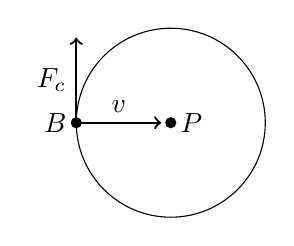
\begin{tikzpicture}[scale=1.2]
                \draw (0,0) circle (1cm);
                \draw[fill] (0,0) circle (1.5pt) node[anchor=west] {$P$};
                \draw[fill] (-1,0) circle (1.5pt) node[anchor=east] {$B$};
                \draw[thick,->] (-1,0) -- ++(0:0.9cm) node[pos=0.5,anchor=south] {$v$};
                \draw[thick,->] (-1,0) -- ++(90:0.9cm) node[pos=0.5,anchor=east] {$F_c$};
            \end{tikzpicture}
        }
        \wrongchoice{
            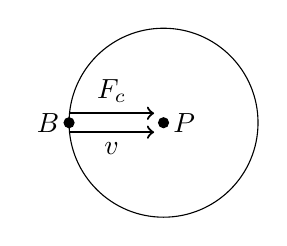
\begin{tikzpicture}[scale=1.2]
                \draw (0,0) circle (1cm);
                \draw[fill] (0,0) circle (1.5pt) node[anchor=west] {$P$};
                \draw[fill] (-1,0) circle (1.5pt) node[anchor=east] {$B$};
                \draw[thick,->] (-1,0) ++(90:0.1cm) -- ++(0:0.9cm) node[pos=0.5,anchor=south] {$F_c$};
                \draw[thick,->] (-1,0) ++(270:0.1cm) -- ++(0:0.9cm) node[pos=0.5,anchor=north] {$v$};
            \end{tikzpicture}
        }
        \correctchoice{
            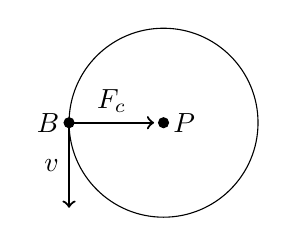
\begin{tikzpicture}[scale=1.2]
                \draw (0,0) circle (1cm);
                \draw[fill] (0,0) circle (1.5pt) node[anchor=west] {$P$};
                \draw[fill] (-1,0) circle (1.5pt) node[anchor=east] {$B$};
                \draw[thick,->] (-1,0) -- ++(0:0.9cm) node[pos=0.5,anchor=south] {$F_c$};
                \draw[thick,->] (-1,0) -- ++(270:0.9cm) node[pos=0.5,anchor=east] {$v$};
            \end{tikzpicture}
        }
        \wrongchoice{
            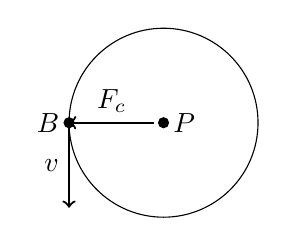
\begin{tikzpicture}[scale=1.2]
                \draw (0,0) circle (1cm);
                \draw[fill] (0,0) circle (1.5pt) node[anchor=west] {$P$};
                \draw[fill] (-1,0) circle (1.5pt) node[anchor=east] {$B$};
                \draw[thick,<-] (-1,0) -- ++(0:0.9cm) node[pos=0.5,anchor=south] {$F_c$};
                \draw[thick,->] (-1,0) -- ++(270:0.9cm) node[pos=0.5,anchor=east] {$v$};
            \end{tikzpicture}
        }
    \end{choices}
    \end{multicols}
\end{question}
}

%% Section June2013
%%--------------------


%% Section June2012
%%--------------------
\element{nysed}{
\begin{question}{June2012-Q09}
    An unbalanced force of \SI{40}{\newton} keeps a \SI{5.0}{\kilo\gram} object traveling in a circle of radius \SI{2.0}{\meter}.
    What is the speed of the object?
    \begin{multicols}{2}
    \begin{choices}
        \wrongchoice{\SI{8.0}{\meter\per\second}}
        \wrongchoice{\SI{2.0}{\meter\per\second}}
        \wrongchoice{\SI{16}{\meter\per\second}}
      \correctchoice{\SI{4.0}{\meter\per\second}}
    \end{choices}
    \end{multicols}
\end{question}
}

\element{nysed}{
\begin{question}{June2012-Q16}
    A stone on the end of a string is whirled clockwise at constant speed in a horizontal circle as shown in the diagram below.
    \begin{center}
    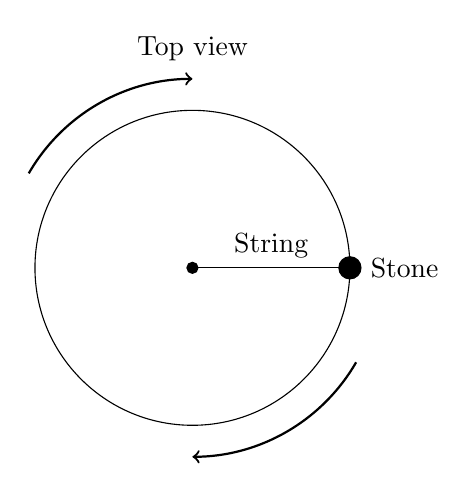
\begin{tikzpicture}
        %% Loop
        \draw (0,0) circle (2cm);
        \draw[fill] (0,0) circle (2pt);
        \draw[fill] (2,0) circle (4pt) node[anchor=west,xshift=4pt] {Stone};
        \draw (0,0) -- (2,0) node[pos=0.5,anchor=south] {String};
        %% Direction
        \draw[thick,->] (330:2.4) arc(330:270:2.4);
        \draw[thick,->] (150:2.4) arc(150:90:2.4);
        %% Label
        \node[anchor=south] at (0,2.5) {Top view};
    \end{tikzpicture}
    \end{center}
    Which pair of arrows best represents the directions of the stone's velocity, $v$,
        and acceleration, $a$, at the position shown?
    \begin{multicols}{2}
    \begin{choices}[o]
        \AMCboxDimensions{down=-1.4cm}
        \wrongchoice{
            \begin{tikzpicture}
                \draw[thin,dotted] (-1.5,-1.5) rectangle (1.5,1.5);
                \draw[very thick,->] (-0.5,1) -- (-0.5,-1)
                    node[pos=0.5,anchor=west] {$\vec{v}$};
                \draw[very thick,->] (0.5,1) -- (0.5,-1)
                    node[pos=0.5,anchor=west] {$\vec{a}$};
            \end{tikzpicture}
        }
        \wrongchoice{
            \begin{tikzpicture}
                \draw[thin,dotted] (-1.5,-1.5) rectangle (1.5,1.5);
                \draw[very thick,->] (0.5,0) -- (-1.5,0)
                    node[pos=0.5,anchor=south] {$\vec{v}$};
                \draw[very thick,->] (1,1) -- (1,-1)
                    node[pos=0.5,anchor=west] {$\vec{a}$};
            \end{tikzpicture}
        }
        \wrongchoice{
            \begin{tikzpicture}
                \draw[thin,dotted] (-1.5,-1.5) rectangle (1.5,1.5);
                \draw[very thick,->] (-1,1) -- (-1,-1)
                    node[pos=0.5,anchor=east] {$\vec{v}$};
                \draw[very thick,->] (-0.5,0) -- (1.5,0)
                    node[pos=0.5,anchor=south] {$\vec{a}$};
            \end{tikzpicture}
        }
        \correctchoice{
            \begin{tikzpicture}
                \draw[thin,dotted] (-1.5,-1.5) rectangle (1.5,1.5);
                \draw[very thick,->] (-1,1) -- (-1,-1)
                    node[pos=0.5,anchor=east] {$\vec{v}$};
                \draw[very thick,->] (1.5,0) -- (-0.5,0)
                    node[pos=0.5,anchor=south] {$\vec{a}$};
            \end{tikzpicture}
        }
    \end{choices}
    \end{multicols}
\end{question}
}

\element{nysed}{
\begin{question}{June2012-Q37}
    A student on an amusement park ride moves in a circular path with radius \SI{3.5}{\meter} once every \SI{8.9}{\second}.
    The student moves at an average speed of:
    \begin{multicols}{2}
    \begin{choices}
        \wrongchoice{\SI{0.39}{\meter\per\second}}
        \wrongchoice{\SI{1.2}{\meter\per\second}}
      \correctchoice{\SI{2.5}{\meter\per\second}}
        \wrongchoice{\SI{4.3}{\meter\per\second}}
    \end{choices}
    \end{multicols}
\end{question}
}


%% Section June2011
%%--------------------
\element{nysed}{
\begin{question}{June2011-Q07}
    The magnitude of the centripetal force acting on an object traveling in a horizontal,
        circular path will \emph{decrease} if the:
    \begin{choices}
      \correctchoice{radius of the path is increased.}
        \wrongchoice{mass of the object is increased.}
        \wrongchoice{direction of motion of the object is reversed.}
        \wrongchoice{speed of the object is increased.}
    \end{choices}
\end{question}
}


%% Section June2010
%%--------------------
\element{nysed}{
\begin{question}{June2010-Q12}
    The diagram below represents a mass, $m$, being swung clockwise at constant speed in a horizontal circle.
    \begin{center}
    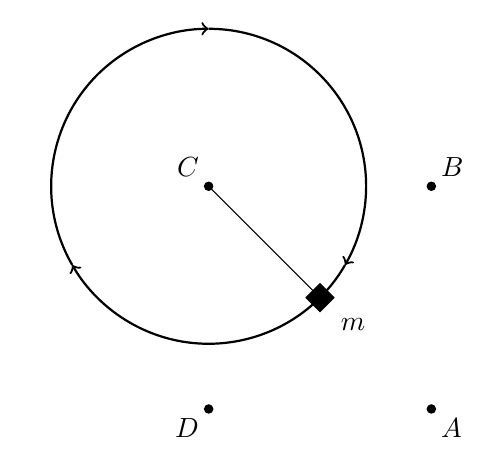
\begin{tikzpicture}
        %% Path
        \draw[thick,->] (90:2) arc (90:-30:2);
        \draw[thick,->] (-30:2) arc (-30:-150:2);
        \draw[thick,->] (-150:2) arc (-150:-270:2);
        %% Block
        \node[minimum size=0.25cm,draw,fill,rotate=45] at (-45:2) {};
        \node[anchor=north west] at (-45:2.2) {$m$};
        \draw (0,0) -- (-45:2);
        %% Points
        \draw[fill] (0,0) circle (1.5pt) node[anchor=south east] {$C$};
        \draw[fill] (-45:2) ++(45:2) circle (1.5pt) node[anchor=south west] {$B$};
        \draw[fill] (-45:2) ++(225:2) circle (1.5pt) node[anchor=north east] {$D$};
        \draw[fill] (-45:2) ++(315:2) circle (1.5pt) node[anchor=north west] {$A$};
    \end{tikzpicture}
    \end{center}
    At the instance shown, the centripetal force acting on mass $m$ is directed toward point:
    \begin{multicols}{4}
    \begin{choices}[o]
        \wrongchoice{$A$}
        \wrongchoice{$B$}
      \correctchoice{$C$}
        \wrongchoice{$D$}
    \end{choices}
    \end{multicols}
\end{question}
}


%% Section June2009
%%--------------------
\element{nysed}{
\begin{question}{June2009-Q07}
    A go-cart travels around a flat, horizontal circular track with radius of \SI{25}{\meter}.
    The mass of the go-cart with the rider is \SI{200}{\kilo\gram}.
    The magnitude of the maximum centripetal force exerted by the track on the go-cart is \SI{1200}{\newton}.
    What is the maximum speed the \SI{200}{\kilo\gram} go-cart can travel without sliding off the track?
    \begin{multicols}{2}
    \begin{choices}
        \wrongchoice{\SI{8.0}{\meter\per\second}}
      \correctchoice{\SI{12}{\meter\per\second}}
        \wrongchoice{\SI{150}{\meter\per\second}}
        \wrongchoice{\SI{170}{\meter\per\second}}
    \end{choices}
    \end{multicols}
\end{question}
}

\element{nysed}{
\begin{question}{June2009-Q08}
    A go-cart travels around a flat, horizontal circular track with radius of \SI{25}{\meter}.
    The mass of the go-cart with the rider is \SI{200}{\kilo\gram}.
    The magnitude of the maximum centripetal force exerted by the track on the go-cart is \SI{1200}{\newton}.
    Which change would increase the maximum speed at which the go-cart could travel without sliding off this track?
    \begin{choices}
        \wrongchoice{Decrease the coefficient of friction between the go-cart and the track.}
        \wrongchoice{Decrease the radius of the track.}
      \correctchoice{Increase the radius of the track.}
        \wrongchoice{Increase the mass of the go-cart.}
    \end{choices}
\end{question}
}


%% Section Jan2009
%%--------------------
\element{nysed}{
\begin{question}{Jan2009-Q07}
    Centripetal force $F_c$ acts on a car going around a curve.
    If the speed of the car were twice as great,
        the magnitude of the centripetal force necessary to keep the car moving in the same path would be:
    \begin{multicols}{4}
    \begin{choices}
        \wrongchoice{$F_c$}
        \wrongchoice{$2 F_c$}
        \wrongchoice{$\dfrac{F_c}{2}$}
      \correctchoice{$4 F_c$}
    \end{choices}
    \end{multicols}
\end{question}
}


%% Section June2008
%%--------------------
\element{nysed}{
\begin{question}{June2008-Q10}
    The diagram below shows an object moving counterclockwise around a horizontal,
        circular track.
    \begin{center}
    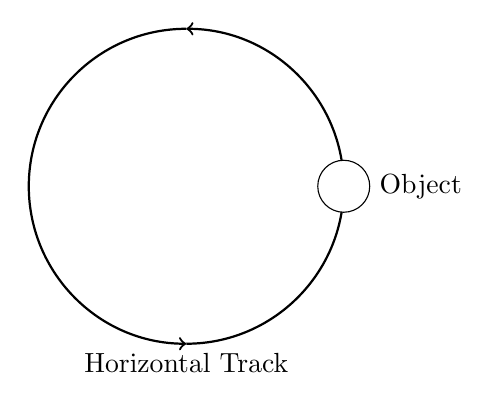
\begin{tikzpicture}
        \draw[thick,->] (0,2) arc (90:270:2cm);
        \draw[thick,->] (0,-2) arc (-90:90:2cm);
        \draw[fill=white] (2,0) circle (0.33cm) node[anchor=west,xshift=0.33cm] {Object};
        \node[anchor=north] at (0,-2) {Horizontal Track};
    \end{tikzpicture}
    \end{center}
    Which diagram represents the direction of both the object's velocity and the centripetal force acting on the object when it is in the position shown?
    \begin{multicols}{2}
    \begin{choices}
        \AMCboxDimensions{down=-0.75cm}
        \small
        \wrongchoice{
            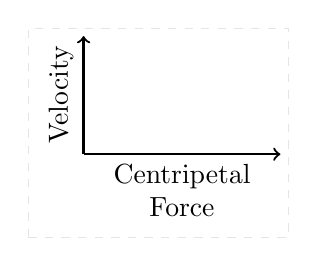
\begin{tikzpicture}
                \draw[white!90!black,dashed] (-2em,-3em) rectangle (2.6,1.6);
                \draw[thick,->] (0,0) -- (0,1.5) node[pos=0.5,rotate=90,anchor=south] {Velocity};
                \draw[thick,->] (0,0) -- (2.5,0) node[pos=0.5,anchor=north,text width=6em,text centered] {Centripetal Force};
            \end{tikzpicture}
        }
        \correctchoice{
            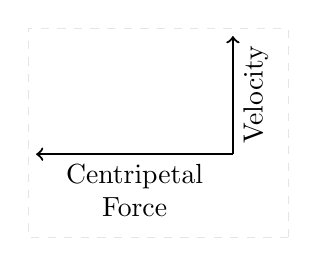
\begin{tikzpicture}
                \draw[white!90!black,dashed] (+2em,-3em) rectangle (-2.6,1.6);
                \draw[thick,->] (0,0) -- (0,1.5) node[pos=0.5,rotate=90,anchor=north] {Velocity};
                \draw[thick,->] (0,0) -- (-2.5,0) node[pos=0.5,anchor=north,text width=6em,text centered] {Centripetal Force};
            \end{tikzpicture}
        }
        \wrongchoice{
            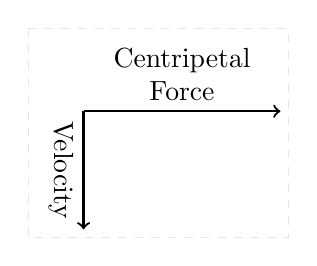
\begin{tikzpicture}
                \draw[white!90!black,dashed] (-2em,+3em) rectangle (+2.6,-1.6);
                \draw[thick,->] (0,0) -- (0,-1.5) node[pos=0.5,rotate=-90,anchor=north] {Velocity};
                \draw[thick,->] (0,0) -- (2.5,0) node[pos=0.5,anchor=south,text width=6em,text centered] {Centripetal Force};
            \end{tikzpicture}
        }
        \wrongchoice{
            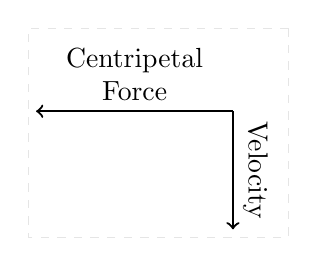
\begin{tikzpicture}
                \draw[white!90!black,dashed] (+2em,+3em) rectangle (-2.6,-1.6);
                \draw[thick,->] (0,0) -- (0,-1.5) node[pos=0.5,rotate=-90,anchor=south] {Velocity};
                \draw[thick,->] (0,0) -- (-2.5,0) node[pos=0.5,anchor=south,text width=6em,text centered] {Centripetal Force};
            \end{tikzpicture}
        }
    \end{choices}
    \end{multicols}
\end{question}
}

\element{nysed}{
\begin{question}{June2008-Q13}
    A \SI{1750}{\kilo\gram} car travels at a constant speed of \SI{15.0}{\meter\per\second} around a horizontal,
        circular track with radius of \SI{45}{\meter}.
    The magnitude of the centripetal force acting on the car is:
    \begin{multicols}{2}
    \begin{choices}
        \wrongchoice{\SI{5.00}{\newton}}
        \wrongchoice{\SI{583}{\newton}}
      \correctchoice{\SI{48750}{\newton}}
        \wrongchoice{\SI{3.94e5}{\newton}}
    \end{choices}
    \end{multicols}
\end{question}
}

\element{nysed}{
\begin{question}{June2008-Q42}
    Which graph best represents the relationship between the magnitude of the centripetal acceleration and the speed of an object moving in a circle of constant radius?
    \begin{multicols}{2}
    \begin{choices}
        \AMCboxDimensions{down=-2.5em}
        \correctchoice{
            \begin{tikzpicture}
                \begin{axis}[
                    axis y line=left,
                    axis x line=bottom,
                    axis line style={->},
                    xlabel={speed},
                    xtick=\empty,
                    ylabel={acceleration},
                    ytick=\empty,
                    xmin=0,xmax=11,
                    ymin=0,ymax=11,
                    width=\columnwidth,
                    very thin,
                ]
                \addplot[line width=1pt,domain=0:10]{0.1*x*x};
                \end{axis}
            \end{tikzpicture}
        }
        \wrongchoice{
            \begin{tikzpicture}
                \begin{axis}[
                    axis y line=left,
                    axis x line=bottom,
                    axis line style={->},
                    xlabel={speed},
                    xtick=\empty,
                    ylabel={acceleration},
                    ytick=\empty,
                    xmin=0,xmax=11,
                    ymin=0,ymax=11,
                    width=\columnwidth,
                    very thin,
                ]
                \addplot[line width=1pt,domain=0:10]{x};
                \end{axis}
            \end{tikzpicture}
        }
        \wrongchoice{
            \begin{tikzpicture}
                \begin{axis}[
                    axis y line=left,
                    axis x line=bottom,
                    axis line style={->},
                    xlabel={speed},
                    xtick=\empty,
                    ylabel={acceleration},
                    ytick=\empty,
                    xmin=0,xmax=11,
                    ymin=0,ymax=11,
                    width=\columnwidth,
                    very thin,
                ]
                \addplot[line width=1pt,domain=0:10]{10/x};
                \end{axis}
            \end{tikzpicture}
        }
        \wrongchoice{
            \begin{tikzpicture}
                \begin{axis}[
                    axis y line=left,
                    axis x line=bottom,
                    axis line style={->},
                    xlabel={speed},
                    xtick=\empty,
                    ylabel={acceleration},
                    ytick=\empty,
                    xmin=0,xmax=11,
                    ymin=0,ymax=11,
                    width=\columnwidth,
                    very thin,
                ]
                \addplot[line width=1pt,domain=0:10]{8};
                \end{axis}
            \end{tikzpicture}
        }
    \end{choices}
    \end{multicols}
\end{question}
}


%% Section Jan2008
%%--------------------
\element{nysed}{
\begin{question}{Jan2008-Q10}
    A car rounds a horizontal curve of constant radius at a constant speed.
    Which diagram best represents the directions of both the car's velocity, $v$, and acceleration, $a$?
    \begin{multicols}{2}
    \begin{choices}
        \AMCboxDimensions{down=-1cm}
        \wrongchoice{
            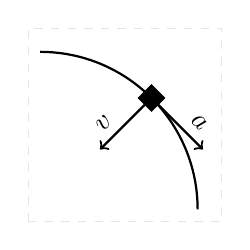
\begin{tikzpicture}
                \draw[dashed,white!90!black] (-1ex,-1ex) rectangle (2.3,2.3);
                \draw[thick] (0:2) arc (0:90:2);
                \node[minimum width=0.25,minimum height=0.15,draw,fill,rotate=-45] (A) at (45:2) {};
                \draw[thick,->] (A.east) -- ++(315:0.8) node[pos=0.66,anchor=south,rotate=-45] {$a$};
                \draw[thick,->] (A.south) -- ++(225:0.8) node[pos=0.66,anchor=south,rotate=45] {$v$};
            \end{tikzpicture}
        }
        \wrongchoice{
            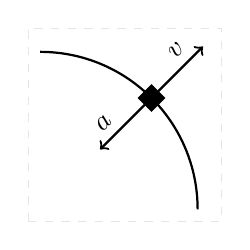
\begin{tikzpicture}
                \draw[dashed,white!90!black] (-1ex,-1ex) rectangle (2.3,2.3);
                \draw[thick] (0:2) arc (0:90:2);
                \node[minimum width=0.25,minimum height=0.15,draw,fill,rotate=-45] (A) at (45:2) {};
                \draw[thick,->] (A.south) -- ++(225:0.8) node[pos=0.66,anchor=south,rotate=45] {$a$};
                \draw[thick,->] (A.north) -- ++(45:0.8) node[pos=0.66,anchor=south,rotate=45] {$v$};
            \end{tikzpicture}
        }
        \correctchoice{
            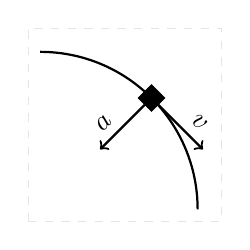
\begin{tikzpicture}
                \draw[dashed,white!90!black] (-1ex,-1ex) rectangle (2.3,2.3);
                \draw[thick] (0:2) arc (0:90:2);
                \node[minimum width=0.25,minimum height=0.15,draw,fill,rotate=-45] (A) at (45:2) {};
                \draw[thick,->] (A.south) -- ++(225:0.8) node[pos=0.66,anchor=south,rotate=45] {$a$};
                \draw[thick,->] (A.east) -- ++(315:0.8) node[pos=0.66,anchor=south,rotate=-45] {$v$};
            \end{tikzpicture}
        }
        \wrongchoice{
            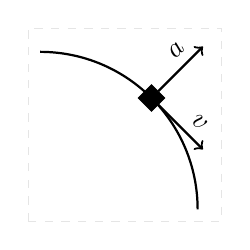
\begin{tikzpicture}
                \draw[dashed,white!90!black] (-1ex,-1ex) rectangle (2.3,2.3);
                \draw[thick] (0:2) arc (0:90:2);
                \node[minimum width=0.25,minimum height=0.15,draw,fill,rotate=-45] (A) at (45:2) {};
                \draw[thick,->] (A.north) -- ++(45:0.8) node[pos=0.66,anchor=south,rotate=45] {$a$};
                \draw[thick,->] (A.east) -- ++(315:0.8) node[pos=0.66,anchor=south,rotate=-45] {$v$};
            \end{tikzpicture}
        }
    \end{choices}
    \end{multicols}
\end{question}
}


%% Section June2007
%%--------------------
\element{nysed}{
\begin{question}{June2007-Q04}
    A car moves with constant speed in a clockwise direction around a circular path of radius $r$,
        as represented in the diagram below.
    \begin{center}
    \includegraphics[keepaspectratio,scale=0.66]{June2007-Q04}
    %\begin{tikzpicture}
    %% NOTE: tikz
    %\end{tikzpicture}
    \end{center}
    When the car is in the position shown,
        its acceleration is directed toward the:
    \begin{multicols}{2}
    \begin{choices}
      \correctchoice{east}
        \wrongchoice{west}
        \wrongchoice{south}
        \wrongchoice{north}
    \end{choices}
    \end{multicols}
\end{question}
}

\element{nysed}{
\begin{question}{Jan2007-Q06}
    A ball attached to a string is moved at constant speed in a horizontal circular path.
    A target is located near the path of the ball as shown in the diagram.
    \begin{center}
    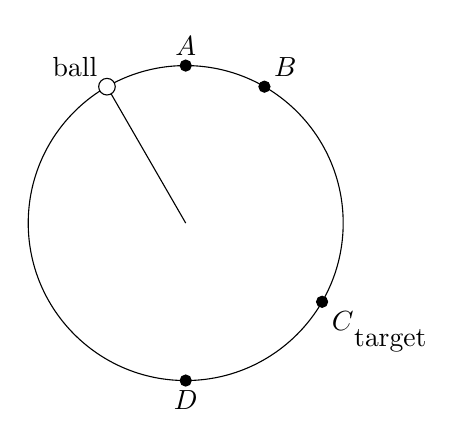
\begin{tikzpicture}
        %% Circle
        \draw (0,0) circle (2cm);
        %% Ball and string
        \draw[] (0:0cm) -- (120:2cm) node[anchor=south east] {ball};
        \draw[fill=white] (120:2cm) circle (3pt);
        %% Labels
        \draw[fill] (90:2cm) circle (2pt) node[anchor=south] {$A$};
        \draw[fill] (60:2cm) circle (2pt) node[anchor=south west] {$B$};
        \draw[fill] (-30:2cm) circle (2pt) node[anchor=north west] {$C$};
        \draw[fill] (270:2cm) circle (2pt) node[anchor=north] {$D$};
        %% Target
        %% NOTE: TODO: TARGET NOT finished
        \node[] at (-30:3cm) {target};
        %\draw rectangle
    \end{tikzpicture}
    \end{center}
    At which point along the ball's path should the string be released,
        if the ball is to hit the target?
    \begin{multicols}{4}
    \begin{choices}[o]
        \wrongchoice{$A$}
      \correctchoice{$B$}
        \wrongchoice{$C$}
        \wrongchoice{$D$}
    \end{choices}
    \end{multicols}
\end{question}
}

\element{nysed}{
\begin{question}{June2007-Q08}
    A \SI{0.50}{\kilo\gram} object moves in a horizontal circular path with a radius of \SI{0.25}{\meter} at a constant speed of \SI{4.0}{\meter\per\second}.
    What is the magnitude of the object's acceleration?
    \begin{multicols}{2}
    \begin{choices}
      \correctchoice{\SI{64}{\meter\per\second}}
        \wrongchoice{\SI{8.0}{\meter\per\second}}
        \wrongchoice{\SI{32}{\meter\per\second}}
        \wrongchoice{\SI{16}{\meter\per\second}}
    \end{choices}
    \end{multicols}
\end{question}
}


%% Section Jan2007
%%--------------------


%% Section June2006
%%--------------------
\element{nysed}{
\begin{question}{June2006-Q07}
    The diagram below shows the top view of a \SI{65}{\kilo\gram} student at point $A$ on an amusement park ride.
    The ride spins the student in a horizontal circle of radius \SI{2.5}{\meter}, at a constant speed of \SI{8.6}{\meter\per\second}.
    The floor is lowered and the student remains against the wall without falling to the floor.
    \begin{center}
        \includegraphics[keepaspectratio,scale=0.8]{June2006-Q07}
    \end{center}
    Which vector best represents the direction of the centripetal acceleration of the student at point $A$?
    \begin{multicols}{2}
    \begin{choices}
        \AMCboxDimensions{down=-0.4cm}
        \correctchoice{
            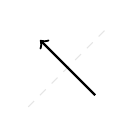
\begin{tikzpicture}
                \draw[dashed,white!90!black] (0,0) -- (1,1);
                \draw[thick,->] (0.85,0.15) -- (0.15,0.85);
            \end{tikzpicture}
        }
        \wrongchoice{
            \begin{tikzpicture}
                \draw[dashed,white!90!black] (0,0) -- (1,1);
                \draw[thick,->] (0.85,0.85) -- (0.15,0.15);
            \end{tikzpicture}
        }
        \wrongchoice{
            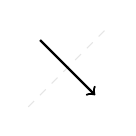
\begin{tikzpicture}
                \draw[dashed,white!90!black] (0,0) -- (1,1);
                \draw[thick,->] (0.15,0.85) -- (0.85,0.15);
            \end{tikzpicture}
        }
        \wrongchoice{
            \begin{tikzpicture}
                \draw[dashed,white!90!black] (0,0) -- (1,1);
                \draw[thick,->] (0.15,0.15) -- (0.85,0.85);
            \end{tikzpicture}
        }
    \end{choices}
    \end{multicols}
\end{question}
}

\element{nysed}{
\begin{question}{June2006-Q08}
    The diagram below shows the top view of a \SI{65}{\kilo\gram} student at point $A$ on an amusement park ride.
    The ride spins the student in a horizontal circle of radius \SI{2.5}{\meter}, at a constant speed of \SI{8.6}{\meter\per\second}.
    The floor is lowered and the student remains against the wall without falling to the floor.
    \begin{center}
        \includegraphics[keepaspectratio,scale=0.8]{June2006-Q07}
    \end{center}
    The magnitude of the centripetal force acting on the student at point $A$ is approximately:
    \begin{multicols}{2}
    \begin{choices}
      \correctchoice{\SI{1.9e3}{\newton}}
        \wrongchoice{\SI{1.2e4}{\newton}}
        \wrongchoice{\SI{2.2e2}{\newton}}
        \wrongchoice{\SI{3.0e1}{\newton}}
    \end{choices}
    \end{multicols}
\end{question}
}


%% Section Jan2006
%%--------------------
\element{nysed}{
\begin{question}{Jan2006-Q14}
    The diagram below shows a \SI{5.0}{\kilo\gram} bucket of water being swung in a horizontal circle of \SI{0.70}{\meter} radius at a constant speed of \SI{2.0}{\meter\per\second}
    \begin{center}
        \includegraphics[keepaspectratio,scale=0.75]{Jan2006-Q14}
    \end{center}
    The magnitude of the centripetal force on the buck of water is approximately:
    \begin{multicols}{2}
    \begin{choices}
      \correctchoice{\SI{29}{\newton}}
        \wrongchoice{\SI{14}{\newton}}
        \wrongchoice{\SI{5.7}{\newton}}
        \wrongchoice{\SI{200}{\newton}}
    \end{choices}
    \end{multicols}
\end{question}
}

\element{nysed}{
\begin{question}{Jan2006-Q40}
    In the diagram below, a cart travels clockwise at constant speed in a horizontal circle.
    \begin{center}
        %% NOTE: tikzpicture
        \includegraphics[keepaspectratio,scale=0.8]{Jan2006-Q40}
    \end{center}
    At the position shown in the diagram,
        which arrow indicates the direction of the centripetal acceleration?
    \begin{multicols}{2}
    \begin{choices}
      \correctchoice{$A$}
        \wrongchoice{$B$}
        \wrongchoice{$C$}
        \wrongchoice{$D$}
    \end{choices}
    \end{multicols}
\end{question}
}


%% Section June2005
%%--------------------
\element{nysed}{
\begin{question}{June2005-Q38}
    In the diagram below, $S$ is a point on a car tire rotating at a constant rate.
    \begin{center}
        \includegraphics[keepaspectratio,scale=0.8]{June2005-Q38}
    \end{center}
    Which graph best represents the magnitude of the centripetal acceleration of point $S$ as a function of time?
    \begin{multicols}{2}
    \begin{choices}
        \AMCboxDimensions{down=-2.5em}
        \correctchoice{
            \begin{tikzpicture}
                \begin{axis}[
                    axis y line=left,
                    axis x line=bottom,
                    axis line style={->},
                    xlabel={time},
                    xtick=\empty,
                    ylabel={acceleration},
                    ytick=\empty,
                    xmin=0,xmax=11,
                    ymin=0,ymax=11,
                    width=\columnwidth,
                    very thin,
                ]
                \addplot[line width=1pt,domain=0:10]{8};
                \end{axis}
            \end{tikzpicture}
        }
        \wrongchoice{
            \begin{tikzpicture}
                \begin{axis}[
                    axis y line=left,
                    axis x line=bottom,
                    axis line style={->},
                    xlabel={time},
                    xtick=\empty,
                    ylabel={acceleration},
                    ytick=\empty,
                    xmin=0,xmax=11,
                    ymin=0,ymax=11,
                    width=\columnwidth,
                    very thin,
                ]
                \addplot[line width=1pt,domain=0:10]{x};
                \end{axis}
            \end{tikzpicture}
        }
        \wrongchoice{
            \begin{tikzpicture}
                \begin{axis}[
                    axis y line=left,
                    axis x line=bottom,
                    axis line style={->},
                    xlabel={time},
                    xtick=\empty,
                    ylabel={acceleration},
                    ytick=\empty,
                    xmin=0,xmax=11,
                    ymin=0,ymax=11,
                    width=\columnwidth,
                    very thin,
                ]
                \addplot[line width=1pt,domain=0:10]{5/x};
                \end{axis}
            \end{tikzpicture}
        }
        \wrongchoice{
            \begin{tikzpicture}
                \begin{axis}[
                    axis y line=left,
                    axis x line=bottom,
                    axis line style={->},
                    xlabel={time},
                    xtick=\empty,
                    ylabel={acceleration},
                    ytick=\empty,
                    xmin=0,xmax=11,
                    ymin=0,ymax=11,
                    width=\columnwidth,
                    very thin,
                ]
                \addplot[line width=1pt,domain=0:10]{10 - 0.1*(10-x)*(10-x)};
                \end{axis}
            \end{tikzpicture}
        }
    \end{choices}
    \end{multicols}
\end{question}
}

\element{nysed}{
\begin{question}{June2005-Q46}
    A \SI{1.0e3}{\kilo\gram} car travels at a constant speed of \SI{20}{\meter\per\second} around a horizontal circular track.
    Which diagram correctly represents the direction of the car's velocity ($v$) and the direction of the centripetal force ($F_e$) acting on the car at one particular moment?
    \begin{multicols}{2}
    \begin{choices}
        %% NOTE: tikzpicture
      \correctchoice{\includegraphics[keepaspectratio,scale=0.66]{June2005-Q46-A}}
        \wrongchoice{\includegraphics[keepaspectratio,scale=0.66]{June2005-Q46-B}}
        \wrongchoice{\includegraphics[keepaspectratio,scale=0.66]{June2005-Q46-C}}
        \wrongchoice{\includegraphics[keepaspectratio,scale=0.66]{June2005-Q46-D}}
    \end{choices}
    \end{multicols}
\end{question}
}


%% Section Jan2005
%%--------------------


%% Section June2004
%%--------------------


%% Section Jan2004
%%--------------------
\element{nysed}{
\begin{question}{Jan2004-Q08}
    $A$ ball of mass $M$ at the end of a string is swung in a horizontal circular path of radius $R$ at constant speed $V$.
    Which combination of changes would require the greatest increase in the centripetal force acting on the ball?
    \begin{choices}
        \wrongchoice{doubling $V$ and doubling $R$}
      \correctchoice{doubling $V$ and halving $R$}
        \wrongchoice{halving $V$ and doubling $R$}
        \wrongchoice{halving $V$ and halving $R$}
    \end{choices}
\end{question}
}


%% Section June2003
%%--------------------
\element{nysed}{
\begin{question}{June2003-Q16}
    A child is riding on merry-go-round.
    As the speed of the merry-go-round is doubled,
        the magnitude of the centripetal force acting on the child:
    \begin{multicols}{2}
    \begin{choices}
      \correctchoice{remains the same}
        \wrongchoice{is doubled}
        \wrongchoice{is halved}
        \wrongchoice{is quadrupled}
    \end{choices}
    \end{multicols}
\end{question}
}


%% Section Jan2003
%%--------------------
\element{nysed}{
\begin{question}{Jan2003-Q09}
    A \SI{2.0e3}{\kilo\gram} car travels at a constant speed of \SI{12}{\meter\per\second} around a circular curve of radius \SI{30}{\meter}.
    What is the magnitude of the centripetal acceleration of the car as it goes around the curve?
    \begin{multicols}{2}
    \begin{choices}
      \correctchoice{\SI{4.8}{\meter\per\second\squared}}
        \wrongchoice{\SI{0.40}{\meter\per\second\squared}}
        \wrongchoice{\SI{800}{\meter\per\second\squared}}
        \wrongchoice{\SI{9600}{\meter\per\second\squared}}
    \end{choices}
    \end{multicols}
\end{question}
}

\element{nysed}{
\begin{question}{Jan2003-Q10}
    A \SI{2.0e3}{\kilo\gram} car travels at a constant speed of \SI{12}{\meter\per\second} around a circular curve of radius \SI{30}{\meter}.
    As the car goes around the curve, the centripetal force is directed:
    \begin{choices}
      \correctchoice{toward the center of the circular curve}
        \wrongchoice{away from the center of the circular curve}
        \wrongchoice{tangent to the curve in the direction of motion}
        \wrongchoice{tangent to the curve opposite the direction of motion}
    \end{choices}
\end{question}
}


%% Section Aug2002
%%--------------------
\element{nysed}{
\begin{question}{Aug2002-Q04}
    The diagram below represents a \SI{0.4}{\kilo\gram} stone attached to a string.
    The stone is moving at a constant speed of \SI{4.0}{\meter\per\second} in a horizontal circle having a radius of \SI{0.8}{\meter}.
    \begin{center}
    %% TODO: NOTE: insert graphic
    \begin{tikzpicture}
        \draw[thick,dashed] (0,0) circle (2cm);
        %\draw[thick,->] (170:2cm) arc (170:170:2cm);
        \draw[thick] (0,0) -- (160:2cm)
            node[pos=0.5,anchor=south west] {$r=\SI{0.80}{\meter}$};
        \draw[fill] (160:2cm) circle (4pt);
        \draw[thick,->] (160:2cm) -- ++(250:0.75cm);
        \node[anchor=south] at (-3.2,0.7) {$m=\SI{0.40}{\kilo\gram}$};
        \node[anchor=north] at (-3.2,0.7) {$v=\SI{4.0}{\meter\per\second}$};
    \end{tikzpicture}
    \end{center}
    The magnitude of the centripetal acceleration of the stone is:
    \begin{multicols}{2}
    \begin{choices}
        \wrongchoice{\SI{0.0}{\meter\per\second\squared}}
        \wrongchoice{\SI{2.0}{\meter\per\second\squared}}
        \wrongchoice{\SI{5.0}{\meter\per\second\squared}}
      \correctchoice{\SI{20}{\meter\per\second\squared}}
    \end{choices}
    \end{multicols}
\end{question}
}


%% Section June2002
%%--------------------
\element{nysed}{
\begin{question}{June2002-Q08}
    The diagram shows a student seated on a rotating circular platform,
    holding a \SI{2.0}{\kilo\gram} block with a spring scale.
    The block is \SI{1.2}{\meter} from the center of the platform.
    The block has a constant speed of \SI{8.0}{\meter\per\second}.
    [Frictional forces on the block are negligible.]
    \begin{center}
        \includegraphics[keepaspectratio,scale=1.0]{June2002-Q08}
    \end{center}
    Which statement best describes the block's movement as the platform rotates?
    \begin{choices}
      \correctchoice{Its velocity is directed tangent to the circular path, with an inward acceleration.}
        \wrongchoice{Its velocity is directed tangent to the circular path, with an outward acceleration.}
        \wrongchoice{Its velocity is directed perpendicular to the circular path, with an inward acceleration.}
        \wrongchoice{Its velocity is directed perpendicular to the circular path, with an outward acceleration.}
    \end{choices}
\end{question}
}

\element{nysed}{
\begin{question}{June2002-Q09}
    The diagram shows a student seated on a rotating circular platform,
    holding a \SI{2.0}{\kilo\gram} block with a spring scale.
    The block is \SI{1.2}{\meter} from the center of the platform.
    The block has a constant speed of \SI{8.0}{\meter\per\second}.
    [Frictional forces on the block are negligible.]
    \begin{center}
        \includegraphics[keepaspectratio,scale=1.0]{June2002-Q08}
    \end{center}
    The reading on the spring scale is approximately:
    \begin{multicols}{2}
    \begin{choices}
        \wrongchoice{\SI{20}{\newton}}
      \correctchoice{\SI{110}{\newton}}
        \wrongchoice{\SI{53}{\newton}}
        \wrongchoice{\SI{130}{\newton}}
    \end{choices}
    \end{multicols}
\end{question}
}


%% Section Jan2002
%%--------------------
\element{nysed}{
\begin{question}{Jan2002-Q59}
    A \SI{60}{\kilo\gram} car travels clockwise in a horizontal circle of radius \SI{10}{\meter} at \SI{5.0}{\meter\per\second}.
    \begin{center}
        \includegraphics[keepaspectratio,scale=0.8]{Jan2002-Q59}
    \end{center}
    The centripetal acceleration of the car at the position shown is directed toward point:
    \begin{multicols}{2}
    \begin{choices}[o]
        \wrongchoice{$A$}
        \wrongchoice{$B$}
      \correctchoice{$C$}
        \wrongchoice{$D$}
    \end{choices}
    \end{multicols}
\end{question}
}

\element{nysed}{
\begin{question}{Jan2002-Q60}
    A \SI{60}{\kilo\gram} car travels clockwise in a horizontal circle of radius \SI{10}{\meter} at \SI{5.0}{\meter\per\second}.
    \begin{center}
        \includegraphics[keepaspectratio,scale=0.8]{Jan2002-Q59}
    \end{center}
    The magnitude of the centripetal force acting on the car is:
    \begin{multicols}{2}
    \begin{choices}
        \wrongchoice{\SI{590}{\newton}}
      \correctchoice{\SI{150}{\newton}}
        \wrongchoice{\SI{30}{\newton}}
        \wrongchoice{\SI{2.5}{\newton}}
    \end{choices}
    \end{multicols}
\end{question}
}


%% Section June2001
%%--------------------
\element{nysed}{
\begin{question}{June2001-Q60}
    A \SI{1200}{\kilo\gram} car traveling at a constant speed of \SI{9.0}{\meter\per\second} turns at an intersection.
    The car follows a horizontal circular path with a radius of \SI{25}{\meter} to point $P$.
    \begin{center}
        \includegraphics[keepaspectratio,scale=0.9]{June2001-Q60}
    \end{center}
    The magnitude of the centripetal force acting on the car as it travels around the circular path is approximately:
    \begin{multicols}{2}
    \begin{choices}
        \wrongchoice{\SI{1.1e4}{\newton}}
        \wrongchoice{\SI{1.2e4}{\newton}}
      \correctchoice{\SI{3.9e3}{\newton}}
        \wrongchoice{\SI{4.3e2}{\newton}}
    \end{choices}
    \end{multicols}
\end{question}
}

\element{nysed}{
\begin{question}{June2001-Q61}
    A \SI{1200}{\kilo\gram} car traveling at a constant speed of \SI{9.0}{\meter\per\second} turns at an intersection.
    The car follows a horizontal circular path with a radius of \SI{25}{\meter} to point $P$.
    \begin{center}
        \includegraphics[keepaspectratio,scale=0.9]{June2001-Q60}
    \end{center}
    At point $P$, the car hits an area of ice and loses all frictional force on its tires.
    Which path does the car follow on the ice?
    \begin{multicols}{4}
    \begin{choices}[o]
        \wrongchoice{$A$}
      \correctchoice{$B$}
        \wrongchoice{$C$}
        \wrongchoice{$D$}
    \end{choices}
    \end{multicols}
\end{question}
}

\element{nysed}{
\begin{question}{June2001-Q62}
    An amusement park ride moves a rider at a constant speed of \SI{14}{\meter\per\second} in a horizontal circular path of radius \SI{10}{\meter}.
    What is the rider's centripetal acceleration in terms of $g$,
        the acceleration due to gravity?
    \begin{multicols}{4}
    \begin{choices}
        \wrongchoice{$1g$}
      \correctchoice{$2g$}
        \wrongchoice{$3g$}
        \wrongchoice{$0g$}
    \end{choices}
    \end{multicols}
\end{question}
}


%% Section Jan2001
%%--------------------
\element{nysed}{
\begin{question}{Jan2001-Q56}
    A \SI{1.00e3}{\kilo\gram} car is driven clockwise around a flat circular track of radius \SI{25.0}{\meter}.
    The speed of the car is a constant \SI{5.00}{\meter\per\second}.
    \begin{center}
        \includegraphics[keepaspectratio,scale=0.8]{Jan2001-Q56}
    \end{center}
    What minimum friction force must exist between the tires and the road to prevent the car from skidding as it rounds the curve?
    \begin{multicols}{2}
    \begin{choices}
        \wrongchoice{\SI{1.25e5}{\newton}}
        \wrongchoice{\SI{9.80e4}{\newton}}
        \wrongchoice{\SI{5.00e3}{\newton}}
      \correctchoice{\SI{1.00e3}{\newton}}
    \end{choices}
    \end{multicols}
\end{question}
}

\element{nysed}{
\begin{question}{Jan2001-Q57}
    A \SI{1.00e3}{\kilo\gram} car is driven clockwise around a flat circular track of radius \SI{25.0}{\meter}.
    The speed of the car is a constant \SI{5.00}{\meter\per\second}.
    \begin{center}
        \includegraphics[keepaspectratio,scale=0.8]{Jan2001-Q56}
    \end{center}
    If the circular track were to suddenly become frictionless at the instant shown in the diagram,
        the car's direction of travel would be:
    \begin{multicols}{2}
    \begin{choices}
        \wrongchoice{toward E}
      \correctchoice{toward N}
        \wrongchoice{toward W}
        \wrongchoice{a clockwise spiral}
    \end{choices}
    \end{multicols}
\end{question}
}

\element{nysed}{
\begin{question}{Jan2001-Q57}
    A \SI{1.00e3}{\kilo\gram} car is driven clockwise around a flat circular track of radius \SI{25.0}{\meter}.
    The speed of the car is a constant \SI{5.00}{\meter\per\second}.
    \begin{center}
        \includegraphics[keepaspectratio,scale=0.8]{Jan2001-Q56}
    \end{center}
    If the circular track were to suddenly become frictionless at the instant shown in the diagram,
        the car's direction of travel would be:
    \begin{multicols}{2}
    \begin{choices}
        \wrongchoice{toward E}
      \correctchoice{toward N}
        \wrongchoice{toward W}
        \wrongchoice{a clockwise spiral}
    \end{choices}
    \end{multicols}
\end{question}
}

\element{nysed}{
\begin{question}{Jan2001-Q58}
    A \SI{1.00e3}{\kilo\gram} car is driven clockwise around a flat circular track of radius \SI{25.0}{\meter}.
    The speed of the car is a constant \SI{5.00}{\meter\per\second}.
    \begin{center}
        \includegraphics[keepaspectratio,scale=0.8]{Jan2001-Q56}
    \end{center}
    At the instant shown in the diagram,
        the car's centripetal acceleration is directed:
    \begin{multicols}{2}
    \begin{choices}
      \correctchoice{toward E}
        \wrongchoice{toward N}
        \wrongchoice{toward W}
        \wrongchoice{clockwise}
    \end{choices}
    \end{multicols}
\end{question}
}

\element{nysed}{
\begin{question}{Jan2001-Q59}
    A \SI{1.00e3}{\kilo\gram} car is driven clockwise around a flat circular track of radius \SI{25.0}{\meter}.
    The speed of the car is a constant \SI{5.00}{\meter\per\second}.
    \begin{center}
        \includegraphics[keepaspectratio,scale=0.8]{Jan2001-Q56}
    \end{center}
    Which factor, when doubled, would produce the greatest change in the centripetal force acting on the car?
    \begin{multicols}{2}
    \begin{choices}
        \wrongchoice{mass of the car}
        \wrongchoice{radius of the track}
      \correctchoice{velocity of the car}
        \wrongchoice{weight of the car}
    \end{choices}
    \end{multicols}
\end{question}
}


%% Section June2000
%%--------------------
\element{nysed}{
\begin{question}{June2000-Q60}
    As a cart travels around a horizontal circular track,
        the cart \emph{must} undergo a change in:
    \begin{multicols}{2}
    \begin{choices}
      \correctchoice{velocity}
        \wrongchoice{inertia}
        \wrongchoice{speed}
        \wrongchoice{weight}
    \end{choices}
    \end{multicols}
\end{question}
}

\element{nysed}{
\begin{question}{June2000-Q64}
    A ball attached to a string is whirled at a constant speed of \SI{2.0}{\meter\per\second} in a horizontal circle of radius \SI{0.50}{\meter}.
    What is the magnitude of the ball's centripetal acceleration?
    \begin{multicols}{2}
    \begin{choices}
        \wrongchoice{\SI{1.0}{\meter\per\second\squared}}
        \wrongchoice{\SI{2.0}{\meter\per\second\squared}}
      \correctchoice{\SI{8.0}{\meter\per\second\squared}}
        \wrongchoice{\SI{4.0}{\meter\per\second\squared}}
    \end{choices}
    \end{multicols}
\end{question}
}


%% Section June1999
%%--------------------
\newcommand{\JuneNineteenNinetyNineQSixtyThree}{
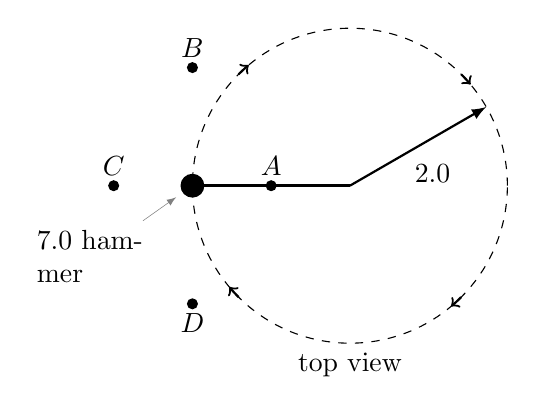
\begin{tikzpicture}
    %% Circle
    \draw[dashed] (0,0) circle (2cm);
    %% Arrows
    \foreach \x in {45,135,225,315} \draw[black,thick,->] (\x:2) arc(\x:{\x-5}:2);
    \draw[thick,-latex] (0,0) -- (30:2) node[pos=0.4,anchor=north west] {\SI{2.0}{\meter}};
    \node[anchor=north] at (0,-2) {top view};
    %% options
    \fill (-2,0) ++(90:1.5) circle (2pt) node[anchor=south] {$B$};
    \fill (-2,0) ++(180:1) circle (2pt) node[anchor=south] {$C$};
    \fill (-2,0) ++(270:1.5) circle (2pt) node[anchor=north] {$D$};
    \fill (-2,0) ++(0:1) circle (2pt) node[anchor=south] {$A$};
    %% Rock and directions
    \fill (180:2) circle (1ex);
    \node[pin={[text width=4em,pin edge={latex-,shorten <=1mm}]225:{\SI{7.0}{\kilo\gram} hammer}}] at (180:2) {};
    \draw[very thick,->] (0,0) -- (180:2);
\end{tikzpicture}
}

\element{nysed}{
\begin{question}{June1999-Q63}
    An athlete in a hammer-throw event swings a \SI{7.0}{\kilo\gram} hammer in a horizontal circle at a constant speed of \SI{12}{\meter\per\second}.
    The radius of the hammer's path is \SI{2.0}{\meter}.
    \begin{center}
        \JuneNineteenNinetyNineQSixtyThree
    \end{center}
    At the position shown,
        the centripetal force acting on the hammer is directed toward point:
    \begin{multicols}{4}
    \begin{choices}[o]
      \correctchoice{$A$}
        \wrongchoice{$B$}
        \wrongchoice{$C$}
        \wrongchoice{$D$}
    \end{choices}
    \end{multicols}
\end{question}
}

\element{nysed}{
\begin{question}{June1999-Q64}
    An athlete in a hammer-throw event swings a \SI{7.0}{\kilo\gram} hammer in a horizontal circle at a constant speed of \SI{12}{\meter\per\second}.
    The radius of the hammer's path is \SI{2.0}{\meter}.
    \begin{center}
        \JuneNineteenNinetyNineQSixtyThree
    \end{center}
    What is the magnitude of the centripetal acceleration of the hammer?
    \begin{multicols}{2}
    \begin{choices}
        \wrongchoice{\SI{6.0}{\meter\per\second\squared}}
        \wrongchoice{\SI{24}{\meter\per\second\squared}}
      \correctchoice{\SI{72}{\meter\per\second\squared}}
        \wrongchoice{\SI{500}{\meter\per\second\squared}}
    \end{choices}
    \end{multicols}
\end{question}
}

\element{nysed}{
\begin{question}{June1999-Q66}
    An athlete in a hammer-throw event swings a \SI{7.0}{\kilo\gram} hammer in a horizontal circle at a constant speed of \SI{12}{\meter\per\second}.
    The radius of the hammer's path is \SI{2.0}{\meter}.
    \begin{center}
        \JuneNineteenNinetyNineQSixtyThree
    \end{center}
    If the hammer is released at the position shown,
        it will travel toward point:
    \begin{multicols}{4}
    \begin{choices}[o]
        \wrongchoice{$A$}
      \correctchoice{$B$}
        \wrongchoice{$C$}
        \wrongchoice{$D$}
    \end{choices}
    \end{multicols}
\end{question}
}


%% Section June1998
%%--------------------

%% NOTE: June1998-Q58 requires graphic, tikz?
%% NOTE: June1998-Q59 same as Q58
%% NOTE: June1998-Q60 same as Q58
\newcommand{\JuneNineteenNinetyNineQFiftyEight}{
\begin{tikzpicture}
    %% path
\end{tikzpicture}
}

\element{nysed}{
\begin{question}{June1998-Q59}
    The diagram below shows a \SI{2.0}{\kilo\gram} cart traveling at a constant speed in a horizontal circle of radius \SI{3.0}{\meter}.
    The magnitude of the centripetal force of the cart is \SI{24}{\newton}.
    \begin{center}
        \JuneNineteenNinetyNineQFiftyEight
    \end{center}
    In the position shown, the acceleration of the cart is:
    \begin{choices}
        \wrongchoice{\SI{8.0}{\meter\per\second\squared} directed toward point $A$}
        \wrongchoice{\SI{8.0}{\meter\per\second\squared} directed toward point $D$}
        \wrongchoice{\SI{12.0}{\meter\per\second\squared} directed toward point $A$}
        \wrongchoice{\SI{12.0}{\meter\per\second\squared} directed toward point $D$}
    \end{choices}
\end{question}
}

\element{nysed}{
\begin{question}{June1998-Q60}
    The diagram below shows a \SI{2.0}{\kilo\gram} cart traveling at a constant speed in a horizontal circle of radius \SI{3.0}{\meter}.
    The magnitude of the centripetal force of the cart is \SI{24}{\newton}.
    \begin{center}
        \JuneNineteenNinetyNineQFiftyEight
    \end{center}
    Which statement correctly describes the direction of the cart's velocity and centripetal force in the position shown?
    \begin{choices}
        \wrongchoice{velocity is directed toward point $B$, and the centripetal force is directed toward point $A$}
        \wrongchoice{velocity is directed toward point $B$, and the centripetal force is directed toward point $D$}
        \wrongchoice{velocity is directed toward point $C$, and the centripetal force is directed toward point $A$}
        \wrongchoice{velocity is directed toward point $C$, and the centripetal force is directed toward point $D$}
    \end{choices}
\end{question}
}

\element{nysed}{
\begin{question}{June1998-Q61}
    The diagram below shows a \SI{2.0}{\kilo\gram} cart traveling at a constant speed in a horizontal circle of radius \SI{3.0}{\meter}.
    The magnitude of the centripetal force of the cart is \SI{24}{\newton}.
    \begin{center}
        \JuneNineteenNinetyNineQFiftyEight
    \end{center}
    What is the speed of the cart?
    \begin{multicols}{2}
    \begin{choices}
        \wrongchoice{\SI{6.0}{\meter\per\second}}
        \wrongchoice{\SI{16}{\meter\per\second}}
        \wrongchoice{\SI{36}{\meter\per\second}}
        \wrongchoice{\SI{4.0}{\meter\per\second}}
    \end{choices}
    \end{multicols}
\end{question}
}


%% Section June1997
%%--------------------
\element{nysed}{
\begin{question}{June1997-Q07}
    A ball rolls through a hollow semicircular tube lying flat on a horizontal tabletop.
    Which diagram shows the path of the ball after emerging from the tube,
        as viewed from above?
    \begin{multicols}{2}
    \begin{choices}
        \AMCboxDimensions{down=-1cm}
        \wrongchoice{
            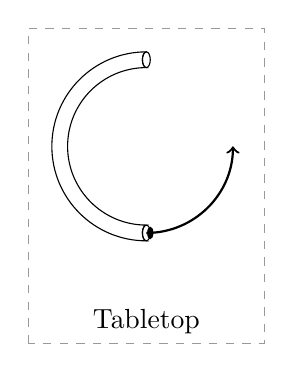
\begin{tikzpicture}
                %% table top
                \draw[dashed,white!60!black] (-1.5,-2.5) rectangle (1.5,1.5);
                \node[anchor=south] at (0,-2.5) {Tabletop};
                %% loop
                \draw (0,1.2) arc (90:270:1.2) arc(270:90:0.05 and 0.1) arc(270:90:1.0) arc(270:90:0.05 and 0.1) -- cycle;
                \draw (0,-1.1) circle (0.05 and 0.1);
                \draw (0,+1.1) circle (0.05 and 0.1);
                %% ball and vector
                \fill (0.05,-1.1) circle (0.04 and 0.08);
                \draw[thick,->] (0,-1.1) arc(270:360:1.1);
            \end{tikzpicture}
        }
        \wrongchoice{
            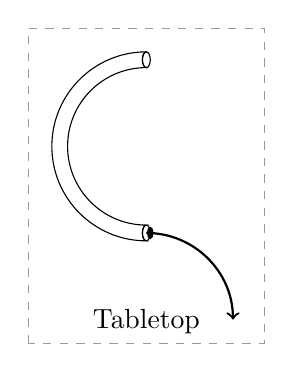
\begin{tikzpicture}
                %% table top
                \draw[dashed,white!60!black] (-1.5,-2.5) rectangle (1.5,1.5);
                \node[anchor=south] at (0,-2.5) {Tabletop};
                %% loop
                \draw (0,1.2) arc (90:270:1.2) arc(270:90:0.05 and 0.1) arc(270:90:1.0) arc(270:90:0.05 and 0.1) -- cycle;
                \draw (0,-1.1) circle (0.05 and 0.1);
                \draw (0,+1.1) circle (0.05 and 0.1);
                %% ball and vector
                \fill (0.05,-1.1) circle (0.04 and 0.08);
                \draw[thick,->] (0,-1.1) arc(90:0:1.1);
            \end{tikzpicture}
        }
        \wrongchoice{
            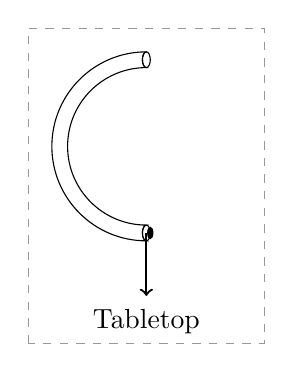
\begin{tikzpicture}
                %% table top
                \draw[dashed,white!60!black] (-1.5,-2.5) rectangle (1.5,1.5);
                \node[anchor=south] at (0,-2.5) {Tabletop};
                %% loop
                \draw (0,1.2) arc (90:270:1.2) arc(270:90:0.05 and 0.1) arc(270:90:1.0) arc(270:90:0.05 and 0.1) -- cycle;
                \draw (0,-1.1) circle (0.05 and 0.1);
                \draw (0,+1.1) circle (0.05 and 0.1);
                %% ball and vector
                \fill (0.05,-1.1) circle (0.04 and 0.08);
                \draw[thick,->] (0,-1.1) -- ++(270:0.8);
            \end{tikzpicture}
        }
        %% Newton's first law
        \correctchoice{
            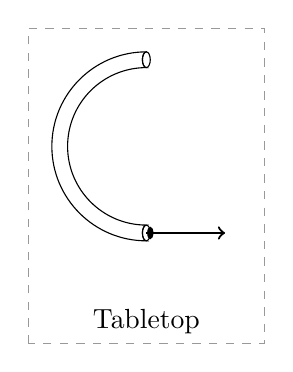
\begin{tikzpicture}
                %% table top
                \draw[dashed,white!60!black] (-1.5,-2.5) rectangle (1.5,1.5);
                \node[anchor=south] at (0,-2.5) {Tabletop};
                %% loop
                \draw (0,1.2) arc (90:270:1.2) arc(270:90:0.05 and 0.1) arc(270:90:1.0) arc(270:90:0.05 and 0.1) -- cycle;
                \draw (0,-1.1) circle (0.05 and 0.1);
                \draw (0,+1.1) circle (0.05 and 0.1);
                %% ball and vector
                \fill (0.05,-1.1) circle (0.04 and 0.08);
                \draw[thick,->] (0,-1.1) -- ++(0:1);
            \end{tikzpicture}
        }
    \end{choices}
    \end{multicols}
\end{question}
}

%% NOTE: Q58 to Q60 uses common graphic
%% NOTE: June1997-Q58 requires graphics
%% NOTE: June1997-Q59 requires graphics
%% NOTE: June1997-Q60 requires graphics


%% Section June1996
%%--------------------
\newcommand{\JuneOneNineNineSixQFiftyNine}{
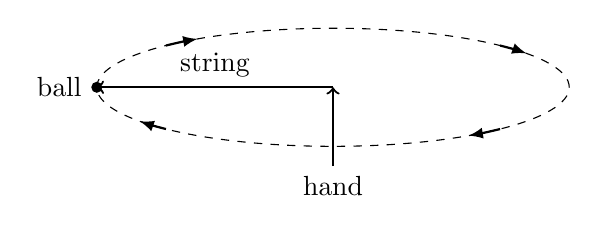
\begin{tikzpicture}
    %% path
    \draw[dashed] (0,0) circle (3cm and 0.75cm);
    \draw[thick,->] (0,0) -- (180:3) node[pos=0.5,anchor=south] {string};
    %% arrows
    \foreach \x in {45,135,225,315}
        \draw[thick,-latex] ({3*cos(\x)},{0.75*sin(\x)}) arc(\x:{\x-10}:3 and 0.75);
    %% ball
    \fill (180:3) circle (2pt) node[anchor=east,xshift=-2pt] {ball};
    %% hand
    \draw[thick,->] (0,-1) -- (0,0) node[pos=0,anchor=north] {hand};
\end{tikzpicture}
}

\element{nysed}{
\begin{question}{June1996-Q59}
    The diagram shows a student spinning a \SI{0.10}{\kilo\gram} ball at the end of a \SI{0.50}{\meter} string in a horizontal circle at a constant speed of \SI{10}{\meter\per\second}.
    [Neglect air resistance.]
    \begin{center}
        %% NOTE: tikz?
        \JuneOneNineNineSixQFiftyNine
    \end{center}
    If the magnitude of the force applied to the string by the student's hand is increased,
        the magnitude of the acceleration of the ball in its circular path will:
    \begin{choices}
        \wrongchoice{decrease}
      \correctchoice{increase}
        \wrongchoice{remain the same}
    \end{choices}
\end{question}
}

\element{nysed}{
\begin{question}{June1996-Q60}
    The diagram shows a student spinning a \SI{0.10}{\kilo\gram} ball at the end of a \SI{0.50}{\meter} string in a horizontal circle at a constant speed of \SI{10}{\meter\per\second}.
    [Neglect air resistance.]
    \begin{center}
        \JuneOneNineNineSixQFiftyNine
    \end{center}
    The magnitude of the centripetal force required to keep the ball in this circular path is:
    \begin{multicols}{2}
    \begin{choices}
        \wrongchoice{\SI{5.0}{\newton}}
        \wrongchoice{\SI{10}{\newton}}
      \correctchoice{\SI{20}{\newton}}
        \wrongchoice{\SI{200}{\newton}}
    \end{choices}
    \end{multicols}
\end{question}
}

\element{nysed}{
\begin{question}{June1996-Q61}
    The diagram shows a student spinning a \SI{0.10}{\kilo\gram} ball at the end of a \SI{0.50}{\meter} string in a horizontal circle at a constant speed of \SI{10}{\meter\per\second}.
    [Neglect air resistance.]
    \begin{center}
        \JuneOneNineNineSixQFiftyNine
    \end{center}
    Which is the best description of the force keeping the ball in the circular path?
    \begin{choices}
      \correctchoice{perpendicular to the circle and directed toward the center of the circle}
        \wrongchoice{perpendicular to the circle and directed away from the center of the circle}
        \wrongchoice{tangent to the circle and directed in the same direction that the ball is moving}
        \wrongchoice{tangent to the circle and directed opposite to the direction that the ball is moving}
    \end{choices}
\end{question}
}

\element{nysed}{
\begin{question}{June1996-Q62}
    A convertible car with its top down is traveling at constant speed around a circular track,
        as shown in the diagram below.
    \begin{center}
    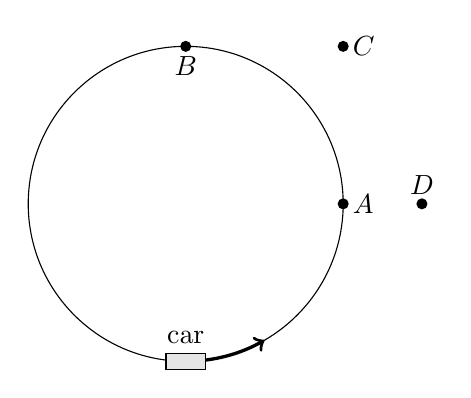
\begin{tikzpicture}
        %% track
        \draw (0,0) circle (2cm);
        %% car
        \draw[very thick,->] (0,-2) arc (270:300:2);
        \draw[fill=white!90!black] (-0.25,-1.9) rectangle (0.25,-2.1);
        \node[anchor=south] at (0,-1.9) {car};
        %% Options
        \fill (2,0) circle (2pt) node[anchor=west] {$A$};
        \fill (2,2) circle (2pt) node[anchor=west] {$C$};
        \fill (0,2) circle (2pt) node[anchor=north] {$B$};
        \fill (3,0) circle (2pt) node[anchor=south] {$D$};
    \end{tikzpicture}
    \end{center}
    When the car is at point $I$, if a passenger in the car throws a ball straight up,
        the ball could land at point:
    \begin{multicols}{4}
    \begin{choices}[o]
        \wrongchoice{$A$}
        \wrongchoice{$B$}
      \correctchoice{$C$}
        \wrongchoice{$D$}
    \end{choices}
    \end{multicols}
\end{question}
}


%% Section June1995
%%--------------------
\newcommand{\nysedJuneNineteenNinetyFiveQFiftyNine}{
\begin{tikzpicture}
    %% clockwise path
    \draw[dashed] (0,0) circle (2cm);
    \draw[thick,-latex] (0,0) -- (135:2) node[pos=0.5,anchor=south,rotate=-45] {\SI{2.0}{\meter}};
    \foreach \x in {100,220,340}
        \draw[thick,-latex] (\x:2) arc(\x:{\x-2}:2);
    %% Cart
    \node[minimum height=1ex,minimum width=0.66ex,draw,fill] (C) at (2,0) {};
    \node[anchor=west] at (C.east) {Cart};
    %% options
    \fill (0,0) circle (2pt) node[anchor=south west] {$Q$};
    \fill (4,0) circle (2pt) node[anchor=south west] {$R$};
    \fill (2,-2) circle (2pt) node[anchor=south west] {$S$};
    \fill (0,-2) circle (2pt) node[anchor=north west] {$P$};
\end{tikzpicture}
}

\element{nysed}{
\begin{question}{June1995-Q59}
    The diagram shows a \SI{5.0}{\kilo\gram} cart traveling clockwise in a horizontal circle of radius \SI{2.0}{\meter} at a constant speed of \SI{4.0}{\meter\per\second}.
    \begin{center}
        \nysedJuneNineteenNinetyFiveQFiftyNine
    \end{center}
    %% start question
    At the position show, the velocity of the cart is directed toward point?
    \begin{multicols}{4}
    \begin{choices}
        \wrongchoice{$P$}
        \wrongchoice{$Q$}
        \wrongchoice{$R$}
      \correctchoice{$S$}
    \end{choices}
    \end{multicols}
\end{question}
}

\element{nysed}{
\begin{question}{June1995-Q60}
    The diagram shows a \SI{5.0}{\kilo\gram} cart traveling clockwise in a horizontal circle of radius \SI{2.0}{\meter} at a constant speed of \SI{4.0}{\meter\per\second}.
    \begin{center}
        \nysedJuneNineteenNinetyFiveQFiftyNine
    \end{center}
    %% start question
    At the position show, the centripetal acceleration of the cart is directed toward point:
    \begin{multicols}{4}
    \begin{choices}
        \wrongchoice{$P$}
      \correctchoice{$Q$}
        \wrongchoice{$R$}
        \wrongchoice{$S$}
    \end{choices}
    \end{multicols}
\end{question}
}

\element{nysed}{
\begin{question}{June1995-Q61}
    The diagram shows a \SI{5.0}{\kilo\gram} cart traveling clockwise in a horizontal circle of radius \SI{2.0}{\meter} at a constant speed of \SI{4.0}{\meter\per\second}.
    \begin{center}
        \nysedJuneNineteenNinetyFiveQFiftyNine
    \end{center}
    %% start question
    If the mass of the cart was doubled,
        the magnitude of the centripetal acceleration of the cart would be:
    \begin{multicols}{2}
    \begin{choices}
      \correctchoice{unchanged}
        \wrongchoice{doubled}
        \wrongchoice{halved}
        \wrongchoice{quadrupled}
    \end{choices}
    \end{multicols}
\end{question}
}

\element{nysed}{
\begin{question}{June1995-Q62}
    The diagram shows a \SI{5.0}{\kilo\gram} cart traveling clockwise in a horizontal circle of radius \SI{2.0}{\meter} at a constant speed of \SI{4.0}{\meter\per\second}.
    \begin{center}
        \nysedJuneNineteenNinetyFiveQFiftyNine
    \end{center}
    %% start question
    What is the magnitude of the centripetal force acting on the cart?
    \begin{multicols}{2}
    \begin{choices}
        \wrongchoice{\SI{8.0}{\newton}}
        \wrongchoice{\SI{20}{\newton}}
      \correctchoice{\SI{40}{\newton}}
        \wrongchoice{\SI{50}{\newton}}
    \end{choices}
    \end{multicols}
\end{question}
}


%% Section June1994
%%--------------------


%% Section June1989
%%--------------------
\element{nysed}{
\begin{question}{June1989-Q62}
    Two masses, $A$ and $B$, move in circular path as shown in the diagram.
    \begin{center}
    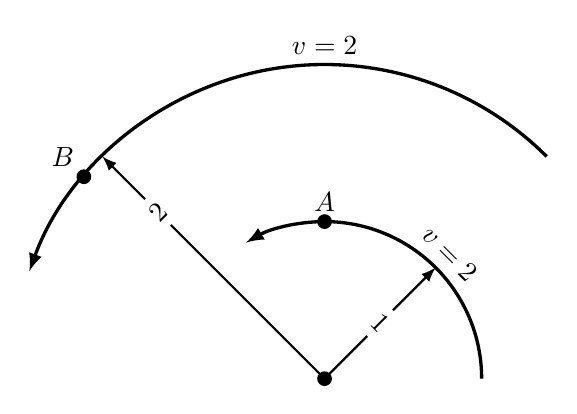
\begin{tikzpicture}[scale=1.33]
        \fill (0,0) circle (2pt);
        %% A loop
        \fill (90:1.5) circle (2pt) node[anchor=south] {$A$};
        \draw[thick,-latex] (0,0) -- (45:1.5) node[pos=0.5,anchor=center,fill=white,rotate=-45] {\SI{1}{\meter}};
        \draw[very thick,-latex] (1.5,0) arc(0:120:1.5) node[pos=0.375,anchor=south,rotate=-45] {$v=\SI{2}{\meter\per\second}$};
        %% B loop
        \fill (140:3) circle (2pt) node[anchor=south east] {$B$};
        \draw[thick,-latex] (0,0) -- (135:3) node[pos=0.75,anchor=center,fill=white,rotate=45] {\SI{2}{\meter}};
        \draw[very thick,-latex] (45:3) arc(45:160:3);
        \node[anchor=south] at (0,3) {$v=\SI{2}{\meter\per\second}$};
    \end{tikzpicture}
    \end{center}
    The centripetal acceleration of mass $A$,
        compared to that of mass $B$, is:
    \begin{choices}
        \wrongchoice{the same}
      \correctchoice{twice as great}
        \wrongchoice{one-half as great}
        \wrongchoice{four times as great}
    \end{choices}
\end{question}
}

\element{nysed}{
\begin{question}{June1989-Q65}
    The diagram below shows an object traveling clockwise in a horizontal,
        circular path at constant speed.
    \begin{center}
    \begin{tikzpicture}
        \fill (0,0) circle (1.5pt);
        %% path
        \draw (0,0) circle (2cm);
        \draw[thick,->] (135:2.5) arc(135:80:2.5);
        \path[postaction={decoration={text along path, text={clockwise},text align=center},decorate}] (135:2.7) arc(135:80:2.7);
        \path[postaction={decoration={text along path, text={motion},text align=center},decorate}] (135:2.1) arc(135:80:2.1);
        %% object
        \draw[fill=white!60!black] (2,0) circle (5pt) node[anchor=west,xshift=5pt] {object};
    \end{tikzpicture}
    \end{center}
    Which arrow best shows the direction of the centripetal acceleration of the object at the instant shown?
    \begin{multicols}{2}
    \begin{choices}
        \AMCboxDimensions{down=-0.8cm}
        \correctchoice{
            \begin{tikzpicture}[scale=2]
                \draw[dashed,white!60!black] (0,0) rectangle (1,1);
                \draw[thick,->] (1,0.5) -- (0,0.5);
            \end{tikzpicture}
        }
        \wrongchoice{
            \begin{tikzpicture}[scale=2]
                \draw[dashed,white!60!black] (0,0) rectangle (1,1);
                \draw[thick,->] (0,0.5) -- (1,0.5);
            \end{tikzpicture}
        }
        \wrongchoice{
            \begin{tikzpicture}[scale=2]
                \draw[dashed,white!60!black] (0,0) rectangle (1,1);
                \draw[thick,->] (0.5,1) -- (0.5,0);
            \end{tikzpicture}
        }
        \wrongchoice{
            \begin{tikzpicture}[scale=2]
                \draw[dashed,white!60!black] (0,0) rectangle (1,1);
                \draw[thick,->] (0.5,0) -- (0.5,1);
            \end{tikzpicture}
        }
    \end{choices}
    \end{multicols}
\end{question}
}


\endinput


